\documentclass[12pt,english]{article}
\usepackage{geometry}
\geometry{verbose,letterpaper,tmargin=2.4cm,bmargin=2.4cm,lmargin=2.4cm,rmargin=2.4cm}
\usepackage[T1]{fontenc}
\usepackage{lmodern}
\usepackage{amssymb,amsmath}
\usepackage{ifxetex,ifluatex}
\usepackage{natbib}
\bibliographystyle{plainnat}
\usepackage{graphicx}
\usepackage{caption}
\usepackage{subcaption}
\usepackage{brush_style}
\usepackage{setspace}
\usepackage{lineno}
\linenumbers
\title{Persistence of marine populations under climate and fishing}
\author{Emma Fuller$^1$, Eleanor Brush$^2$, Malin Pinsky$^{1,3}$}
\date{\small (1): Department of Ecology and Evolutionary Biology, Princeton University, Princeton, New Jersey 08544 USA \\
(2): Program in Quantitative and Computational Biology, Princeton University, Princeton, New Jersey 08544 USA \\
(3): Department of Ecology, Evolution and Natural Resources, Rutgers University, New Brunswick, New Jersey 08901 USA}

\begin{document}
\maketitle
\pagebreak
\begin{spacing}{1.9}
\begin{flushleft}

\section{Abstract}

When the climate changes, so does the location of habitats suitable for an organism's survival and reproduction. This change does not occur in isolation but appears on a background of other disturbances, making the study of interactions between stressors important. In order to understand how two disturbances, range shift and harvesting, interact and affect population persistence, we analyzed an integrodifference model that explicitly includes the mechanisms of dispersal and reproduction. We have shown how the critical rates of harvesting and climate velocity that suffice to drive the population extinct depend on the growth rate and dispersal kernel of the population.  We measured the interaction between the stressors and find the disturbances interact nearly additively in the parameter space that results in a stable population, with low positive synergy present only at the greatest harvest rates and climate velocity.  Using simulations, we introduced two conservation techniques, threshold harvest rules and marine protected areas (MPAs), and have shown that these approaches can be effective management tools as they can mitigate the interaction between the two stressors.  

\hspace{10cm}

\noindent {\bf Keywords:} Climate change, fishing, integrodifference model, synergy, multiple disturbances

\section{Introduction}

A number of stressors can disturb an ecosystem, and ecologists have quantified the consequences of many of these of perturbations \citep{Wilcoveetal1998, Crainetal2008, DarlingCote2008}. Less work, however, has been done to measure the effects of multiple stressors and the interactions between them.  If disturbances interact synergistically, a perturbation that has little effect when occurring individually may amplify the disturbance caused by a coincident perturbation \citep{Crainetal2008, DarlingCote2008,Nyeetal2013,Gurevitchetal2000}.   In the most extreme (and worrying) cases, synergistic interactions between multiple stressors could drive a population extinct even though assessments of impacts individually predict the population to be robust (e.g. \citet{Pelletieretal2006}).  If disturbances interact antagonistically, on the other hand, the effects of multiple stressors may be less than that predicted by the individual effects of the stressors.  Since disturbances rarely occur in isolation, measuring the effects of multiple disturbances gives a better understanding of the likely impacts to the system \citep{DoakMorris2010, Fordhametal2013, Foltetal1999}.


Climate change and fishing, two of the largest human impacts on the ocean \citep{Halpernetal2008}, provide an important example of ecological disturbances occurring in unison. Marine fish are already moving in response to climate change \citep{ Perryetal2005, HiddinkHoftstede2008, Rijnsdorpetal2009, Dulvyetal2008, Simpsonetal2011, Pinskyetal2013} and are projected to continue in the future \citep{Kelletal2005, Mackenzieetal2007}. These shifting species are also subject to harvesting, among other disturbances including pollution, ocean acidification, habitat fragmentation, and invasive species \citep{Wilcoveetal1998, Salaetal2000, MEA2005, Pinskyetal2013, Barryetal1995, Nyeetal2009}. Previous empirical work has found synergistic interactions between overfishing and temperature-driven range shifts \citep{Lingetal2009} and synergistic interactions between warming temperatures, harvesting and connectivity have been identified in microcosm experiments \citep{Moraetal2007}. This empirical work underscores the importance of understanding how range shifts and harvesting interact. 

A common approach to predicting future population distributions has been to use bioclimatic-envelope models (also known as species distribution models -- SDMs). These statistical models typically correlate presence-absence data with biophysical characteristics such as mean or maximum temperature, rainfall, or salinity, to predict how species ranges' will differ under climate change \citep{Elithetal2006, GuisanThuiller2005, GuisanZimmerman2000}. Despite these models' widespread adoption, many authors have criticized SDMs as oversimplified as they lack species interactions, dispersal and reproductive processes \citep{KearneyPorter2009, Zarnetskeetal2012, Robinsonetal2011}.  Recent work on range shifts has addressed some of these gaps by explicitly including dispersal and reproduction \citep{Berestyckietal2009, ZhouKot2011}. However these models only address one disturbance, climate-driven range shifts.

Previous work has considered the joint impacts of climate and fishing, however these studies consider climate fluctuations (large anomalies around the mean) rather than directional shifts in temperature \citep{WaltersParma1996, KingMcFarlane2006}. When studies consider the effects of climate-driven range shifts on fishing, the models are typically case-specific and detailed, integrating multiple drivers and disturbances \citep{Cheungetal2010, Lindegrenetal2010, Brownetal2010, Merinoetal2010, Merinoetal2010b, Plaganyietal2011, Ainsworthetal2011, Zhangetal2011, Barangeetal2011, Howardetal2013}. These predicted impacts are important for management and conservation planning \citep{Allisonetal2009}, but the complexity of these models makes it difficult to  understand the relative importance of particular drivers, disturbances, and interactions (but see \citet{Nyeetal2013} for an approach using ecosystem-level models to discern relative importance of disturbances).

Here we extend a previously studied model \citep{ZhouKot2011} to a fish population subject to climate-driven range shift and harvesting pressure. The model explicitly included reproduction and dispersal, two mechanistic processes central to species' responses to climate and fishing. Previous work has highlighted the importance of these two processes and their vulnerability to climate change \citep{Fordhametal2013, Hastingsetal2005}.  We find the critical harvesting rate and climate velocity that drive the population extinct and how these critical rates depend on one another.   We also show that climate-driven range shifts and fishing interact nearly additively, with low positive synergy at more extreme levels of the stressors.  

We also examine the efficacy of two different types of management strategies: threshold harvesting rules and marine protected areas (MPAs). MPAs are frequently recommended for conservation of biodiversity and improved fisheries yield \citep{Gainesetal2010}, and we evaluate whether MPAs established for those purposes could improve species persistence when habitat shifts rapidly.  Previous work has suggested protected areas can be a key form of climate insurance and can provide stepping stones to help species keep up with a changing environment \citep{Thomasetal2012, Hannahetal2007}.  We find that threshold harvesting rules remove the interaction between harvesting rates and climate velocity and that MPAs can help a species persist with higher harvesting pressure and slightly increase the maximum climate velocity with which a species can keep up.

\section{Methods}

We studied a model of the dynamics of a fish population constrained to a single, one-dimensional habitat patch by their inability to reproduce outside of that area, as introduced by \cite{ZhouKot2011}. This viable habitat patch (hereafter `patch') shifts at a fixed velocity and harvest occurs at each point in space along the entire one-dimensional world.  We first analytically determined the harvesting rate climate velocity that would drive the population extinct (hereafter the critical harvesting rate and critical climate velocity), and then measured synergy by calculating the drop in biomass caused by each stressor both individually and together. We then added threshold harvesting rules and marine protected areas (MPAs) in numerical simulations of the model to determine how these management strategies affect population persistence.

\subsection{The Model }

In the model of \cite{ZhouKot2011}, the adults from the current year produce offspring according to a recruitment function and these offspring disperse across the one-dimensional world according to a dispersal kernel to become the next generation's adults.  We extend this model by additionally subjecting the adults to harvesting before they produce offspring so that only a proportion of the fish survive to reproduce. These processes -- recruitment, harvesting, and dispersal -- are incorporated into an integrodifference model to describe how the population changes over time. If $n_t(x)$ 
is the density of fish at position $x$ at time $t$, then the density of fish at the next generation is given by

\[n_{t+1}(x)=\int^{\frac{L}{2}+ct}_{-\frac{L}{2}+ct}k(x-y)f((1-h)n_t(y))dy \label{integrodifference},\]

\noindent where $h$ is the proportion of adults harvested, $k(x-y)$ is the dispersal kernel giving the probability of a  larva traveling from position $y$ to position $x$, $L$ is the length of the patch, and $c$ is the rate at which it  shifts across space. We used a Beverton-Holt stock-recruitment function for $f(n)$,

\[f(n_t)=\frac{R_0n_t}{1+\left(\frac{R_0-1}{K}\right)n_t}\]  

\noindent  which gives the number of offspring produced by a population of size $n$ (accounting for density dependence). Here $R_0$ is the intrinsic growth rate and $K$ is carrying capacity (see table 1 for a full description of parameters and functions). 

Analyzing this kind of model becomes easier if the dispersal kernel is separable into its dependence on the source of larvae and its dependence on the destination of the larvae, i.e.~if there are functions $a_i, b_i$ such that $k(x- y) = \sum^\infty_{i=1} a_i(x)b_i(y)$.  In our analyses, as in \cite{Latore:1998fk}, we used the separable Gaussian kernel given by

\[k(x-y)=\frac{1}{2\sqrt{D\pi}}e^{\frac{-(x-y)^2}{4D}}.\]

\noindent To derive analytical expressions, we approximated the kernel, as described Appendix A.3, and analytical results for a separable sinusoidal kernel are also described in Appendix A.4.  We used simulations to analyze a Laplace dispersal kernel that is not amenable to this method, as described below.  %% Why did we choose a Laplace for simulations? Why not just do the same for both analytics and simulations? 

At equilibrium, the population will move in a traveling wave, where the density of fish at a given point in space will change but the density of fish at a location relative to the shifting patch will not. The traveling wave $n^*$ must satisfy

\begin{equation}
n^*(\bar{x})=\int^{\frac{L}{2}}_{-\frac{L}{2}}k(\bar{x}+c-\bar{y})f((1-h))n^*(\bar{y}))d
\bar{y}, \label{traveling_pulse}
\end{equation}

\noindent where $\bar{x}\in\left[-\frac{L}{2}, \frac{L}{2}\right]$ describes the position within the patch \citep{ZhouKot2011}. For a separable kernel, the equilibrium traveling pulse $n^*(x)$ must satisfy 

\begin{equation}
n^*(x)=\sum^\infty_{i=1}
a_i(x)\int^{\frac{L}{2}}_{-\frac{L}{2}}b_i(y-c)f((1-h)n^*(y))dy=\sum^\infty_{i=1}m_ia_i(x), \label{separable_integrodifference}
\end{equation}

\noindent where the $m_i$ satisfy the recursive equations

\begin{equation}
m_i=\int^{\frac{L}{2}}_{-\frac{L}{2}}b_i(y-c)f\left((1-h)\sum^\infty_{j=1}m_ja_j(x)\right)
dy. \label{recursive_m}
\end{equation}

\noindent \citep{Latore:1998fk}.

\subsection{Persistence }
If the population is harvested at low enough levels and the climate velocity is slow enough, the population will be able to persist.  There are threshold values of the harvesting rate $h$ and the climate velocity $c$ such that if we increase the parameters beyond these values, the population will be driven extinct.  When the population is extinct, the system is in equilibrium, i.e. there is a `trivial' traveling pulse, $n^*(\bar{x}) = 0$ for all $x \in \left[-\frac{L}{2}, \frac{L}{2}\right]$, which satisfies Equation (\ref{traveling_pulse}).  If a population persists, it must be able to avoid extinction and grow even when small. If the trivial pulse is stable, the system will return to extinction even after the introduction of a small population. If the trivial pulse is unstable, a small population may increase and form a persistent population. Population persistence is therefore equivalent to the trivial traveling pulse being an unstable equilibrium.  We found the critical parameters, $h^*$ and  $c^*$, by finding the parameters that make the trivial pulse unstable.  See Appendix A.1 for details.

Regardless of its exact functional form, the only property of the recruitment function that determines whether or not a population can persist is how quickly recruitment increases when the population size is near (but above) $0$, which is equivalent to the intrinsic growth rate $R_0=f'(0)$.  For each kernel, therefore, the population's ability to persist depends on properties of the population itself -- the expected distance a larva disperses $\langle d \rangle$ and the intrinsic growth rate $R_0$; properties of the environment -- the length of the viable patch $L$ and how quickly the environment shifts $c$; and the harvesting rate $h$.  
For a Gaussian kernel, the critical rates $c^*$ and $h^*$ are those values of $c$ and $h$ such that 

\[R_0(1-h)2\sqrt{2}\exp\left(\frac{-c^2}{8D}\right)\left[\text{erf}\left(\frac{L-c}{2\sqrt{2D}}\right)-\text{erf}\left(\frac{-L-c}{2\sqrt{2D}}\right)\right]=1.\]

We derive a similar expression for a sinusoidal kernel in the Appendix A.4.  For both kernels, we can approximate the critical harvesting proportion by a function that looks like 
\begin{equation*}
h^*\sim1- \frac{1}{R_0}\cdot C(L,R_0)f(\langle d \rangle,c^2,L^2+3c^2),
\end{equation*}
where $C(L,R_0)$ is a decreasing function of the length of the viable patch and the intrinsic growth rate.
   

\subsection{Calculating synergy }

\citet{ZhouKot2011} only considered whether a shifting environment will drive a population extinct.   In order to quantify whether the two stressors interact additively, synergistically, or antagonistically, we found the total biomass of the population when it reached an equilibrium traveling pulse and compared this equilibrium biomass in the presence and absence of each stressor individually or the two stressors together.   Equations (\ref{recursive_m}) and (\ref{separable_integrodifference}) allowed us to numerically find the  total biomass in the equilibrium traveling pulse.


We used $B_0$ to denote the equilibrium biomass 
without either stressor, $B_\text{h}$ the equilibrium biomass with harvesting but a constant environment, $B_\text{c}$ the 
equilibrium biomass with a shifting environment but no harvesting, and $B_\text{hc}$ the equilibrium biomass with 
both stressors. For each stressor or combination of stressors, we found the drop in  biomass caused 
by stressor $s$,

\[E_\text{s}=B_0-B_\text{s}.\]

\noindent If the stressors do not interact, the drop caused by both stressors would be the sum of the drops caused by 
either individually. The synergy is therefore defined as

\[S = E_\text{hc}-\left(E_\text{h}+E_\text{c}\right).\]

\noindent If the stressors aggravate each other, the effect of both stressors is greater than  we would expect from considering either stressor individually and synergy is positive. If the stressors alleviate each other, the effect of both stressors is less than we would expect from considering either stressor individually and synergy is negative. If the effect of both stressors is exactly as expected from considering either stressor individually, there is no interaction and no synergy.

\subsection{Simulations }

We used simulations to extend the basic integrodifference model in two ways that make it analytically intractable. First, we examined the sensitivity of the model to choice of dispersal kernel by using the Laplace dispersal kernel, 

\[ k(x-y)=\frac{1}{2}be^{-b|x-y|},\]

\noindent a commonly used model of larval dispersal \citep{Pinsky:2011fk}.  Second, we implemented two management strategies, threshold rules and MPAs, to examine their effect on population persistence and on the interactions between stressors.  For every simulation we seeded the world with 50 individuals at a single point, as in \cite{ZhouKot2011}. We first ran through 150 generations in order for the population to reach equilibrium without harvesting or climate shift.  We then added harvesting pressure, allowed the population to again reach equilibrium (150 generations), and finally added climate change by moving the viable patch.  We calculated equilibrium biomass as the mean biomass of 300 time steps once the difference in biomass between successive generations was no greater than $0.1$.  

Under the two management strategies, harvesting pressure was implemented differently.  With a threshold rule, we evaluated the population at each point in space to determine how much harvesting should occur. If the population abundance was below the designated threshold, no harvesting occurred. If the population exceeded the threshold, then we harvested all the `surplus' individuals. We introduce networks of MPAs into our simulations by designating segments of space where the harvesting rate was equal to $0$.  MPAs are typically designed to meet either fishery management  or conservation goals \citep{Agardy1994, HollandBrazee1996, Gainesetal2010a}, thus their spacing and size differ.  Fisheries-oriented MPAs are often designed such that they maximize adult spillover into fishable areas by creating many small reserves closely spaced \citep{HastingsBotsford2003,Gaylordetal2005, Gainesetal2010a}. To mimic this management scheme, we implemented MPAs with a length of $\tfrac{1}{3}$ of the average dispersal distance and a distance of $\tfrac{2}{3}$ of the average dispersal distance between them.   Conservation-oriented MPAs seek to reduce adult spillover by creating fewer larger protected areas \citep{HastingsBotsford2006, Gainesetal2010a}.  To mimic this scheme we implemented MPAs with a length of $4$ times the average dispersal distance and a distance of $8$ times the average dispersal distance between them \citep{Lockwoodetal2002}. 

\section{Results}

\subsection{Interactions Between Stressors }
The critical climate velocity and harvest  rate are inversely related.  As the climate velocity shift $c$ increases, the critical harvesting rate $h^*$ decreases (Figure  \ref{baseline}). This means that a harvesting rate that is sustainable in the absence of environmental shift may no longer be sustainable if the environment starts changing. Conversely, as the harvesting rate $h$ increases, the critical climate velocity $c^*$ decreases (Figure \ref{baseline}).  Thus as harvesting pressure increases, it becomes increasingly easy for a shifting environment to drive the population extinct.

When the climate velocity or harvesting pressure exceed their critical rates ($c^*, h^*$ respectively), the biomass of the population at equilibrium will be equal to $0$.  Before the stressors reaches those thresholds, the equilibrium biomass of the population decreases as either the harvesting pressure increases or the environmental shifts more quickly (Figure \ref{baseline}). Our simulations confirm the analytical results with the critical speed $c^*$ declining as the critical harvest rate $h^*$ increases and vice versa (Figure \ref{nomang}).

It is always the case that increasing the intrinsic growth rate, $R_0$, increases the critical climate velocity $c^*$ and the critical harvesting rate $h^*$, since a population that grows more quickly can recover more quickly from losses caused by these disturbances. However, whether or not dispersing farther is better depends on how quickly the environment is shifting (Figure \ref{baseline}). When the environment is shifting slowly, dispersing farther is detrimental since many larvae will disperse too far away from the viable patch. When the environment is shifting quickly, on the other hand, dispersing farther can help the population persist because some larvae will disperse into the space that will become viable shortly in the future.  This affects the critical harvesting rate: at a low climate velocity, we can more severely harvest populations that have a shorter dispersal distance than those that disperse farther, whereas at a high climate velocity, we can more aggressively harvest populations that disperse farther.

We found low levels of positive synergy between the two stressors in our analysis of the Gaussian kernel (Figure \ref{Synergy}).  Where positive synergy exists, a doubly stressed population loses more biomass than we would predict from either stressor individually.  The stressors interact most strongly at high harvest and climate velocity rates, shortly before they drive the population extinct.  However, the synergistic  loss in biomass is very low, meaning that these stressors interact more or less additively.  We found similar analytical results for a sinusoidal dispersal kernel, which indicates that this result is robust to changes in the dispersal kernel.  

\subsection{Management strategies }

Without any management strategies, we found that the more severely we harvest the population, a slower climate velocity will suffice to drive the population extinct. However, when we put thresholds in place, a small population can always escape harvesting pressure and the critical climate velocity $c^*$ no longer depends on the harvesting rate (Figure \ref{management}). In other words, as long as there is some threshold below which harvesting is not allowed, there is a constant critical climate velocity that only depends on the growth rate, length of the viable patch, and average dispersal distance.  

With either type of MPA strategies examined (many small versus few large), the population withstood combinations of higher climate velocities and harvesting rates (Figure \ref{management}).  At lower climate velocities, MPAs spaced more than one average dispersal distance apart resulted in larger fluctuations of population biomass relative to small, closely spaced, MPAs.  As climate velocities increase, for both MPA strategies, the mean population abundance declines but the population experiences less extreme oscillations in abundance.  Since minimum population biomass is increased, the population is a larger buffer to possible extinction in a stochastic environment. 

\section{Discussion}

Understanding interactions among disturbances will help to design management for populations subjected to these stressors. The co-occurrence of climate change-driven range shifts and fishing mean that there is the potential for synergistic interactions, which have been largely unexamined.  Here we have analyzed
 a general model that incorporates dispersal and reproduction to examine how climate and harvesting interact in their effects on species persistence and biomass. 

For each dispersal kernel we studied, we found that the higher the growth rate and the more the mean dispersal distance matches the climate velocity, the better a population can persist under harvesting and climate change.  Further, we found a negative relationship between the critical harvesting rate and the climate velocity.  That is, the more quickly the environment shifts the less harvesting it takes to drive the population extinct.  This is evidence that the stressors interact since each stressor's ability to drive the population extinct depends on the severity of the other stressor. 

To quantify the interaction between the stressors, we measured the synergy between their effects on population biomass.  We found positive synergy between the stressors and that the synergy is greatest in the region of parameter space where the equilibrium biomass is smallest.  We chose to measure the effect of each stressor by the absolute drop in biomass caused by the stressor, and we used the sum of the individual effects for our null prediction of the effect of both stressors, as in \cite{Crainetal2008, DarlingCote2008,Nyeetal2013}.  In general, measuring synergy against an additive null prediction is more conservative than measuring synergy multiplicatively: the presence of additive synergy implies multiplicative synergy, but not vice versa \citep{Crainetal2008, Foltetal1999}.  Since we found small levels of positive additive synergy between the two stressors, other measures of synergy might show even higher levels of interaction. Worryingly, we find the highest synergy in those populations whose persistence is most tenuous.  This means that harvesting levels or climate velocity that are sustainable individually together can drive a population to extinction.  However the drop in biomass caused by both stressors was never much higher than the null prediction, i.e. synergistic effects were quite small.

Despite the absence of synergy in our analysis, whether or not we should assume that synergy is unlikely to exist between climate velocity and harvesting remains to be seen. Synergy between harvesting and the effects of climate change has been identified in experimental populations \citep{Moraetal2007}, and observationally at both the population \citep{Planque:2010uq}, and ecosystem level \citep{Kirby:2009fk,Planque:2010uq}.  Some of the discrepancies may be due to the ways in which climate was measured. In the experimental populations, effects of climate were mimicked by increased temperatures, and organisms were unable to relocate to thermal optima. Synergy was identified between warming and harvesting but not between habitat fragmentation \citep{Moraetal2007}, which may be more similar to the range shift we analyzed in our theoretical model.  While we did find (very) low levels of positive synergy, we did not find as much as predicted from these empirical studies.  However, these previous results are not directly comparable to ours because they focus on different aspects of climate change, e.g. warming temperature \citep{Moraetal2007,Kirby:2009fk} or a more variable climate \citep{Planque:2010uq}.  Additionally, while we can isolate the affects of climate shift and harvesting in our simple analytical model, there are other forces acting on real populations that may produce the observed synergistic effects.

Absence of synergy does not mean absence of effect, and our results suggest that particular combinations of harvesting and climate velocity will affect some species more than others. Species with a higher reproductive rate and a longer average dispersal distance will better track a high climate velocity relative to a species that has a low reproductive rate and short dispersal distance (Figure \ref{baseline}). The finding that a higher reproductive rate can sustain higher climate velocities and harvesting rates is intuitive, especially because harvesting rate and reproductive rate cancel each other out. However it is worth pointing out that a higher reproductive rate can be generated either by shorter generation times or higher fecundity. Finding that species with shorter generation times can better keep up with shifts in climate is in agreement with empirical work which has found that fish which shifted in response to warming in North Sea had faster life histories than non shifting species \citep{Perryetal2005}. While higher reproductive rates improved a population's ability to persist, increasing dispersal distances did not necessarily. At low speeds, we found that a short dispersal dispersal distance improved the maximum harvesting rate a population could sustain while at higher speeds a longer dispersal distance improved the maximum climate velocity in which the population could persist (Figure \ref{baseline}). This is because when climate is shifting slowly, a large dispersal distance sends most offspring ahead of the patch, while with faster climate velocities a long dispersal distance allows the population to make it to the new patch (Figure \ref{baseline}). Thus climate velocity will selectively favor species with dispersal distances best matched to the rate of shift.   

We also examined whether frequently recommended management approaches, MPAs and harvest control rules, ensure species persistence. With these management strategies we found increases in the population's biomass at equilibrium and an improved ability to persist.  We found that a threshold harvesting rule alleviates interactions between the two stressors. Thresholds have this effect as the management approach effectively prevents harvesting of the leading edge, which allows colonization to occur as if these individuals were moving into un-fished areas. It's interesting to note that novel, low abundance species are commonly unregulated in fisheries systems; so in order to decouple the additive effects of harvest and climate change, management would have to reverse this paradigm by allowing no harvest of shifting species until they had become established in new areas.  

Unlike thresholds, MPAs are explicitly spatial.  Previous work has advanced protected areas as a way to help organisms keep pace with range shifts, as well as to ameliorate anthropogenic disturbances like harvesting and habitat fragmentation \citep{Lawleretal2010, Hannahetal2007,Botsfordetal2001, Gaylordetal2005, HastingsBotsford2003,Thomasetal2012}. Our results show that both threshold and MPAs increase the equilibrium biomass at a given climate velocity, which support their use as a tool to ameliorate the effect of climate velocity. However for MPAs the details mater: few, large MPAs caused increased variability at low climate velocities while many smaller MPAs maintained a population bounded farther from extinction. Finally, with sufficiently high harvesting pressure, few, large MPAs rescued populations at intermediate speeds. With intermediate speeds, the population was able to reach a protected area fast enough to avoid extinction, and the protected area was large enough to allow a partial rebuilding of the population before it moved out the other side. However this effect disappears as speed continues to increase, suggesting that understanding the relationship between climate velocity, dispersal distance and reproductive rate are important parameters in designing management strategies effective under both climate change and harvesting pressure. 

The advantage of a simple model like ours is that it is general enough to be applied to a number of systems.  However, this simplistic approach requires that we ignore complexities known to be present in marine fisheries. For example, we do not include Allee effects, so that even if the population shrank to low levels it was possible for it to persist over time. However, with Alee effects we expect qualitatively similar results. An Allee effect would make it harder for populations to colonize new areas and add a threshold below which fishing drives the population to extinction. Thus an Allee effect would change lower the critical harvest rates and climate velocity, but we do not expect the additive nature of the interaction between climate and harvesting to change.  We also did not include age structure in our model. The effects of both harvesting and climate change may be different across different age classes and may destabilize the system in complicated ways, including resonance \citep{Botsfordetal2011, Planqueetal2010}; and we leave this additional complexity for future work. Similarly, we did not include any mechanisms aside from larval dispersal by which the population could keep up with a shifting climate.  Besides these species-specific extensions, this modeling framework could be extended to consider species interactions, especially predator-prey pairs.  By introducing a predatory species, we would be imposing yet another stressor on the focus species \citep{Lingetal2009, Gurevitchetal2000} and we are interested in measuring the interaction between the effects of this stressor and the two we consider here.

Using a simple mechanistic model like the one we present here provides a useful framework for incorporating additional ecological complexities which can mediate species persistence under multiple disturbances. Using this modeling framework as a starting point, we believe exploring how species interactions, age structure, and additional disturbances (e.g. physiological response to temperature) affect population viability will improve our predictions and help us to understand whether species will persist under predicted climate and harvesting regimes. Finally, this work can help make general predictions as to whether specific life histories offer selective advantages over others as harvesting and range shifts increase and highlights the importance of considering stressors in combination as outcomes can deviate from what we would predict in isolation. This is especially true for management strategies which may result in unanticipated effects such as large fluctuations associated with big, distant MPAs shown here. While the management strategies only change harvesting practices and do not directly address the effects of climate change, understanding how they ameliorate synergistic affects between harvesting and range shifts will help to better implement harvesting rules and place protected areas.  This is encouraging evidence that a single set of of management practices may help to protect marine populations from both harvesting and climate change.

\section*{ Acknowledgements}
We thank Catherine Offord and Will Scott for their contributions to an earlier version of this manuscript. 

\end{flushleft}


\bibliography{fish}
\pagebreak

\section{Tables}
\begin{table}[h]
\caption{Table of variables used in the text}
\begin{tabular}{@{}lllllll@{}}
  Variable & Definition
\\\cmidrule{1-1} \cmidrule{2-2}   
$n_t(x)$ & density of fish at position $x$ at time $t$
\\ $n^*(\overline{x})$ & density of fish at equilibrium at position $\overline{x}$ relative to the patch 
\\ $k(x-y)$ & dispersal kernel, the probability of larva traveling from position $y$ to position $x$
\\ $\langle d \rangle $ & expected distance traveled by larva
\\ $f(n)$ & recruitment function, the number of offspring produced by a population of size $n$
\\ $R_0$ & intrinsic growth rate, $R_0=f'(0)$
\\ $h$ & proportion of adults harvested
\\ $L$ & patch length
\\ $c$ & climate velocity
\end{tabular}
\label{variables}
\end{table}

\pagebreak


\section*{Figure Legends}

\noindent {\bf Figure \ref{baseline}}: (a) The critical harvesting rate on the y-axis as a function of the climate velocity on the x-axis.  Black lines correspond to a growth rate of $R_0=3$, red to $R_0=7$, and blue to $R_0=10$.  Solid lines correspond to an average dispersal distance $\langle d \rangle =0.1$ and dashed lines correspond to an average dispersal distance $\langle d \rangle =0.25$.  These results are from an approximated Gaussian dispersal kernel with $L=1$.  (b) 
The equilibrium biomass of the population as a function of the climate velocity on the x-axis and the harvesting rate on the y-axis. These results are from a Gaussian dispersal kernel with parameters $L=1$, $R_0=10$, $\langle d \rangle = 0.5$. 
\hspace{6in}
\hspace{6in}

\noindent {\bf Figure \ref{Synergy}}: Positive synergy between the two stressors.  The x-axis shows the climate velocity, the y-axis shows the harvesting rate, and the color indicates the loss in biomass in the doubly stressed population in excess of the sum of the losses caused by each stressor individually, $E_\text{hc}-E_\text{h}-E_\text{c}$.  This excess loss, on the order of $.05$, is small in comparison to the total biomass, which can be greater than $40$.  These results are from an approximated Gaussian dispersal kernel with parameters $L=1$, $R_0=10$, $\langle d \rangle = 0.5$.
\hspace{6in}

\hspace{6in}

\noindent {\bf Figure \ref{management}}: The equilibrium biomass of the population as a function of the climate velocity on the x-axis and the harvesting rate on the y-axis with and without management strategies.  (a) MPAs (b) Threshold harvesting levels.  These results are from a simulation with a Laplacian dispersal kernel with parameters $L=1$, $R_0=5$, $K=100$, and $\langle d \rangle =2$.
\pagebreak

\section{Figures}

\begin{figure}[htbp]
\begin{subfigure}{3in}
\subcaption{\label{rates}}
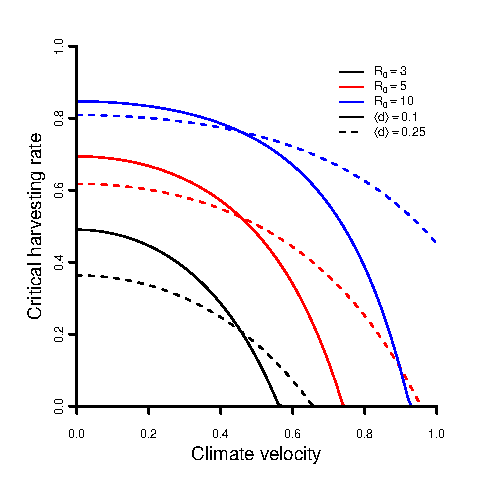
\includegraphics[width=\textwidth]{plots/critical_rates.eps}
\end{subfigure}
\begin{subfigure}{3in}
\subcaption{\label{biomass}}
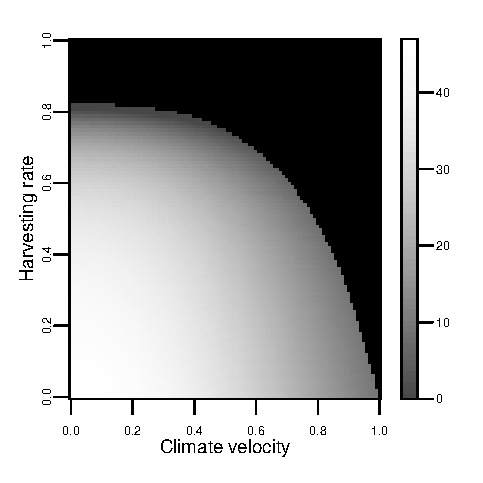
\includegraphics[width=\textwidth]{plots/eqbiomass.eps}
\end{subfigure}

\caption{%(a) The critical harvesting rate on the y-axis as a function of the climate velocity on the x-axis.  Black lines correspond to a growth rate of $R_0=3$, red to $R_0=7$, and blue to $R_0=10$.  Solid lines correspond to an average dispersal distance $\langle d \rangle =0.1$ and dashed lines correspond to an average dispersal distance $\langle d \rangle =0.25$.  (b) The equilibrium biomass of the population as a function of the climate velocity on the x-axis and the harvesting rate on the y-axis. These results are from a Gaussian dispersal kernel with parameters $L=1$, $R_0=5$, $\langle d \rangle = 0.5$.    These results are from an approximated Gaussian dispersal kernel with $L=1$.
}

\label{baseline}
\end{figure}

\pagebreak

\begin{figure}[htbp]
\begin{center}
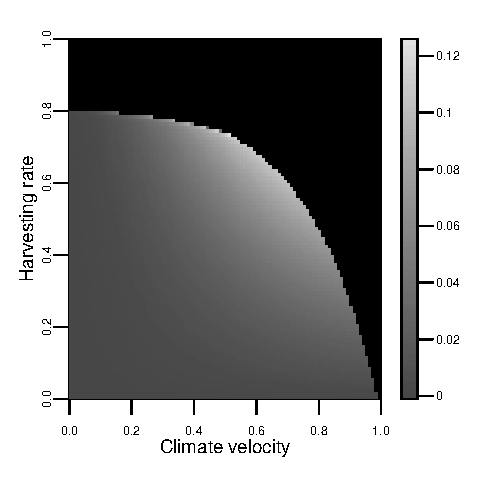
\includegraphics[width=3in]{plots/synergy.eps}
\caption{
%Positive synergy between the two stressors.  The x-axis shows the climate velocity, the y-axis shows the harvesting rate, and the color indicates the loss in biomass in the doubly stressed population in excess of the sum of the losses caused by each stressor individually, $E_\text{hc}-E_\text{h}-E_\text{c}$.  These results are from an approximated Gaussian dispersal kernel with parameters $L=1$, $R_0=5$, $\langle d \rangle = 0.5$.
}
\label{Synergy}
\end{center}
\end{figure}

\pagebreak



\pagebreak

\begin{figure}[htbp]

\begin{subfigure}{.33\textwidth}
\subcaption{}
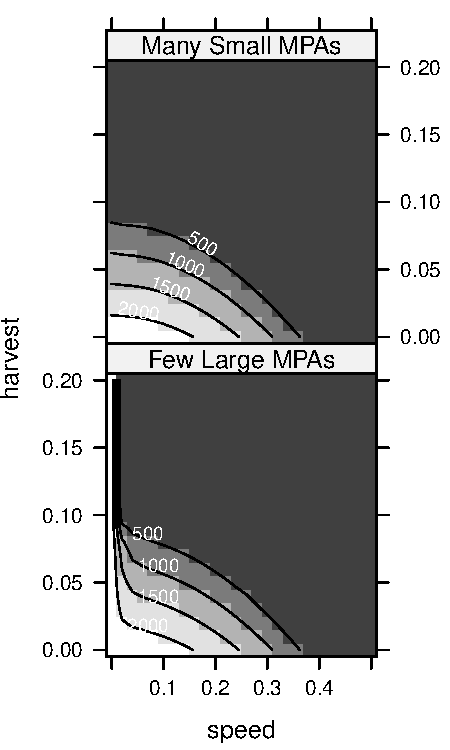
\includegraphics[width=1\textwidth]{plots/MPAs.pdf}
\label{nomang}
\end{subfigure}
\begin{subfigure}{.33\textwidth}
\subcaption{}
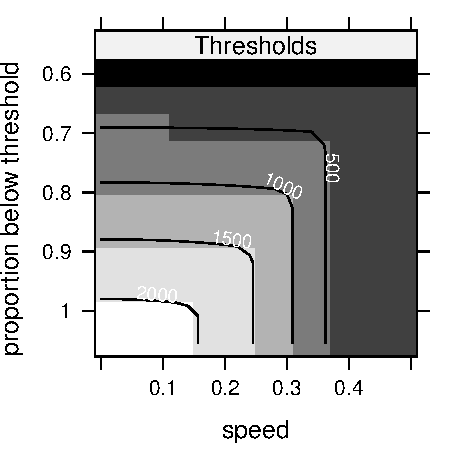
\includegraphics[width=1\textwidth]{plots/Threshold.pdf}
\end{subfigure}
\caption{
%The equilibrium biomass of the population as a function of the climate velocity on the x-axis and the harvesting rate on the y-axis with and without management strategies.  (a) MPAs  (b) Threshold harvesting levels.  These results are from a simulation with a Laplacian dispersal kernel with parameters $L=1$, $R_0=5$, $K=100$, and $\langle d \rangle =2$.
}
\label{management}
\end{figure}


\pagebreak




\end{spacing}
\end{document}
